%\section{Representing Domain Knowledge and Data using Graphs}
The synergy between domain knowledge and data mining can be achieved by employing the RDF model given the fact that RDF allows a combined specification of both schema information and data structured under the schema. In light of Hayes et al's proposal to represent RDF as hypergraphs~\cite{GraphModelRDF}, we develop a set of rules to represent data in transactional tables as hypergraphs or bipartite graphs with minimal loss of semantics. We then propose a novel way to combine the graph representations of data and domain knowledge encoded in ontologies as a unified information source from which valuable insights can be drawn upon.

%RDF's abstract triple syntax has a graph nature. Graphs are mathematical objects that enjoy wide-spread usage for many tasks, which include the visualization and analysis of data for humans, mathematical reasoning, and the implementation as a data structure for developing data mining algorithms. Besides the common graph-theoretic model of RDF as labeled, directed multi-graphs, Hayes has established that RDF can be also represented as hypergraphs (bipartite graphs)~\cite{GraphModelRDF}. This result constitutes an important aspect of the theoretical basis of this dissertation and is discussed in sections below. Furthermore, we develop a set of rules to represent data in transactional tables as hypergraphs or bipartite graphs with minimal loss of semantics. We then propose a novel way to combine the graph representation for domain knowledge and data as a unified information source from which valuable insights can be drawn in a systematic manner.

\section{Graph Representation for Domain Knowledge}
As we have mentioned in Chapter~\ref{chap:background}, graph-based approaches for representing knowledge have long been used in philosophy, psychology, and linguistics. The computer counterpart to this means is the so-called \emph{semantic network} that represents knowledge in patterns of interconnected nodes and arcs which were first developed for artificial intelligence and machine translation~\cite{Sowa91principlesof}. Knowledge such as subsumption hierarchy can be best captured by the semantic network. Distance (similarity) measures can usually be reasonably defined on the network, which is essential in many data mining tasks. In addition, one of the most prominent formalism families among current systems, description logics, have been proven to be successful. Its latest development, OWL, is intended for representing knowledge in the semantic web~\cite{Berners-Lee01}---a giant semantic network that spans the entire Internet. OWL ontologies can be used along with information written in RDF, and OWL ontologies themselves are primarily exchanged as RDF documents. RDF's abstract triple syntax has a graph nature.

We focus on describing various definitions of graph representation models for RDF in this section. The term ``RDF graph" is formally defined as follows according to the W3C specification for RDF semantics~\cite{Hayes_rdf2004}:

\begin{mydef}[\textbf{RDF graph}]
An RDF graph is defined as a set of RDF triples. A subgraph of an RDF graph is a subset of the triples in the graph. A triple is identified with the singleton set containing it, so that each triple in a graph is considered to be a subgraph. A proper subgraph is a proper subset of the triples in the graph. A ground RDF graph is one with no blank nodes.
\end{mydef}

RDF triples can be visualized as a \emph{directed labeled graph} as follows:
\begin{center}\ovalbox{subject} $\stackbin[]{predicate}{\xrightarrow{\hspace*{2cm}}}$ \ovalbox{object}\;,\end{center}
where subjects and objects are represented as nodes, and predicates as edges. The directed labeled graph model for RDF is straightforward and convenient in most cases. But inconsistency arises when using triples to make assertions on predicates. The directed labeled graph model of RDF makes the artificial distinction between resources and properties, which may cause inconsistency in the graph representation. The following example illustrates this point of view.

\begin{figure}[tbh]
\begin{center}
\begin{tabular}{ccc}
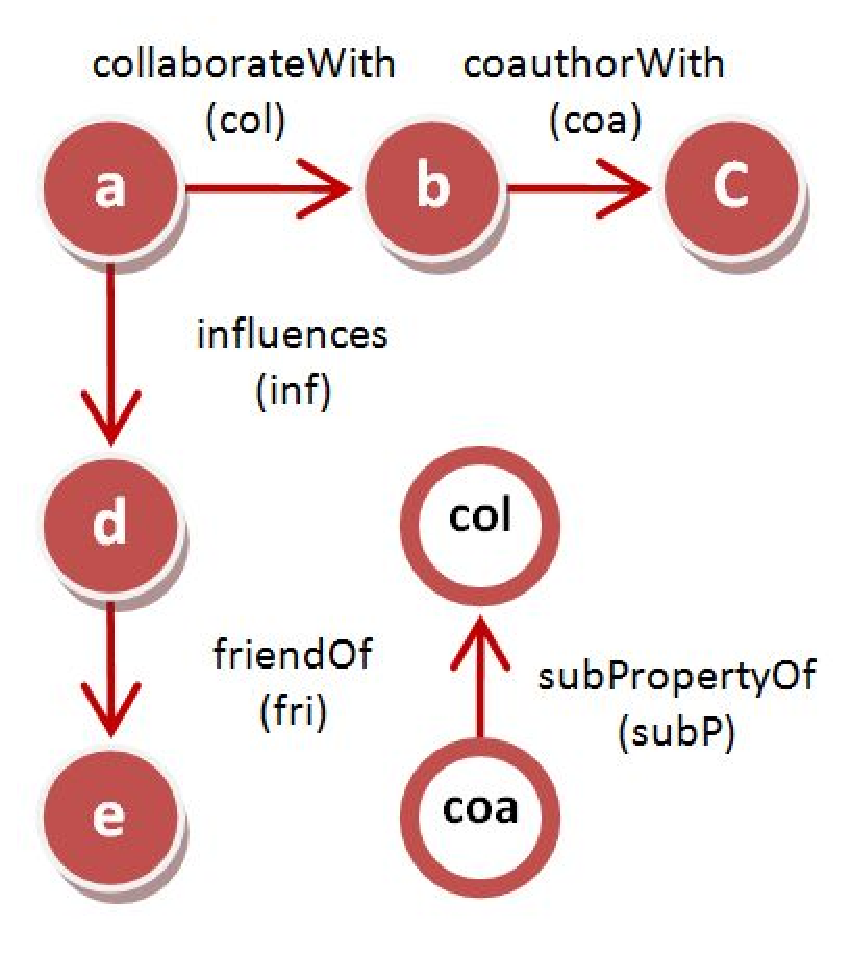
\includegraphics[width=.25\textwidth]{fig/reg_graph.eps} & &
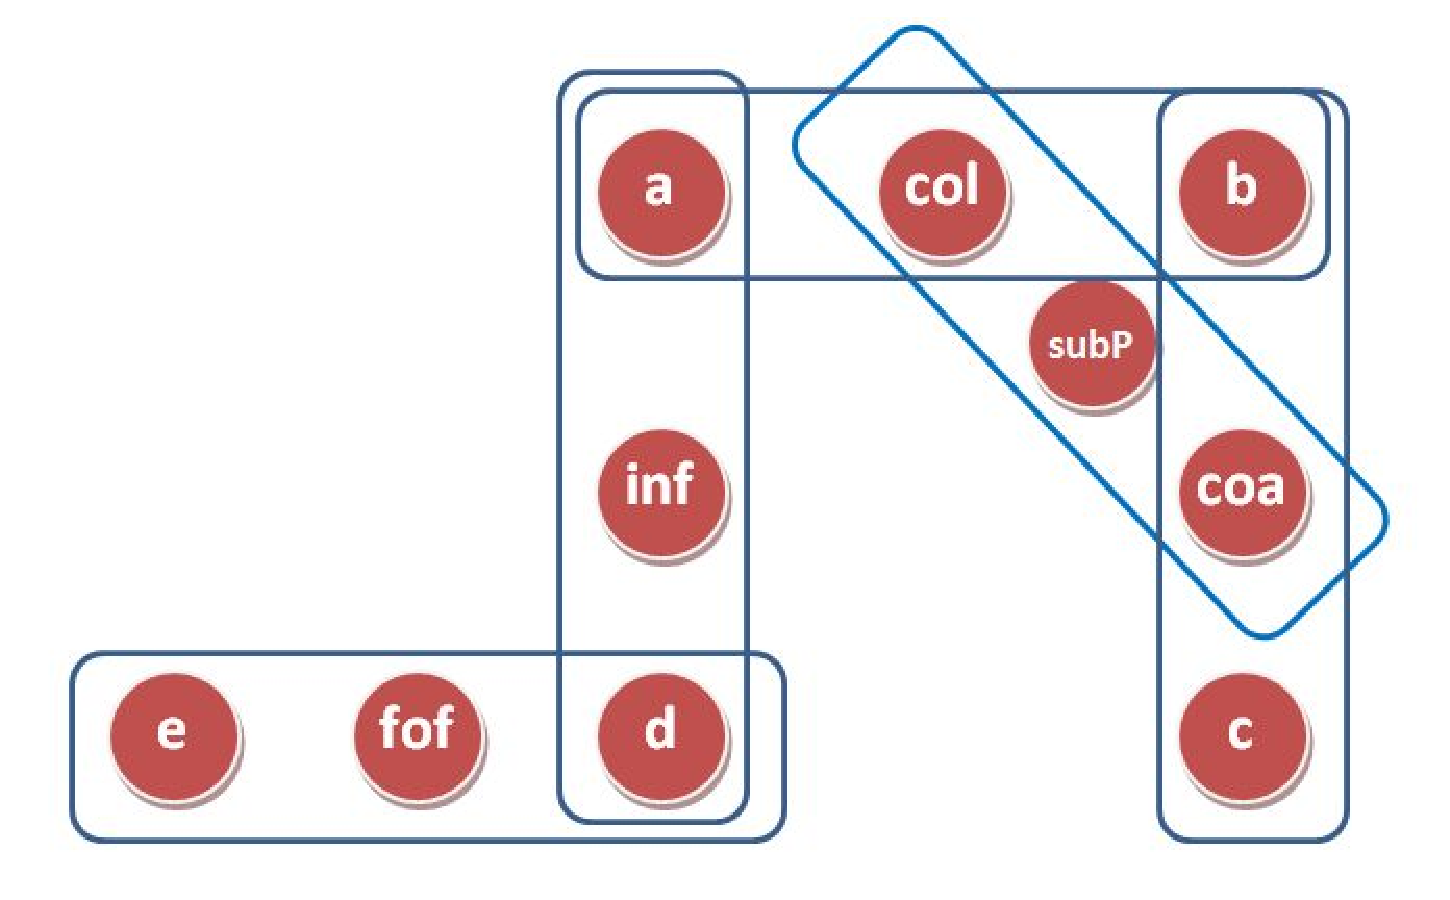
\includegraphics[width=.43\textwidth]{fig/hypergraph.eps}\\
(A) & & (B)\\
\end{tabular}
\end{center}
\caption[A comparison between a simple graph and a hypergraph]{\label{fig:graphcomp} An example of nodes connected by different links, represented by A) a simple graph, and B) a hypergraph.}
\end{figure}

\begin{myexp}[\textbf{Inconsistent representation of the RDF directed labeled graph model}]
\label{ex:inconsistentDG}
In this example, a set of RDF statements is asserted to describe relationships among a group of people. The information expressed includes two different levels, \ie, the meta (ontological) data level and factual data level. The factual data level consists of following statements: $\langle a~ collaborate~ b\rangle$, $\langle b~ coauthor~ c\rangle$, $\langle a~ influence~ d\rangle$ and $\langle d~ friendOf~ e\rangle$. The meta-data level contains one single statement asserting that $coauthor$ is a sub-property of $collaboration$: $\langle coauthor~ subProperty~ collaboration\rangle$. In this case, the representation of $collaboration$ and $coauthor$ is inconsistent --- they are represented as nodes at the factual data level and edges at the meta-data level (see Figure~\ref{fig:graphcomp}(A)).
\end{myexp}

To overcome the inconsistency, Hayes et al.~\cite{GraphModelRDF} proposed to model RDF as a \emph{hypergraph}. A hypergraph~\cite{Hypergraph} is a generalization of a traditional graph where edges, called hyperedges, can connect more than two vertices. If each edge in a hypergraph covers the same number of nodes, it is called $r$-uniform hypergraph, $r$ being the number of nodes on each edge. Any RDF graph can be represented by a simple ordered 3-uniform hypergraph, in which an RDF triple corresponds to a hyperedge, with incident nodes being the subject, predicate and object from the triple. In this way, both meta-data and data level statements can be integrated in a consistent model.
In Fig.~\ref{fig:graphcomp}(B), the information in Example~\ref{ex:inconsistentDG} is represented by a hypergraph and the inconsistency in the directed labeled graph representation is eliminated.
%
%\begin{mydef}[\textbf{Hypergraph}]
%Formally, a hypergraph $G = (V,E)$, is a pair in which $V$ is the vertex set and $E$ is the hyperedge set where each $e \in E$ is a subset of $V$. A weighted hypergraph is a hypergraph that has a positive number $w(e)$ associated with each hyperedge $e$; called the weight of hyperedge $e$: Denote a weighted hypergraph by $G = (V,E,w)$. The degree of a vertex $v \in V$, $d(v)$, is defined as $d(v) = \sum_{v\in V, e\in E}{w(e)}$. The degree of a hyperedge $e$, denoted as $\delta(e)$, is the number of vertices in $e$, i.e. $\delta(e)=|e|$. A hyperedge $e$ is said to be incident with a vertex $v$ when $v \in e$. The hypergraph incidence matrix $\mathbf{H} \in \mathbb{R}^{|V| \times |E|}$ is defined as
%\begin{equation}
%\notag h(v,e)=\left\{\begin{array}{cl}
%	   1, & v \in e \\
%	   0, & otherwise
%	   \end{array}\right.
%\end{equation}
%Throughout the rest of the paper, the diagonal matrix forms for $\delta(e)$, $w(e)$, $d(v)$ are denoted as $\mathbf{D}_e$, $\mathbf{W} \in \mathbb{R}^{|E|}$, and $\mathbf{D}_v \in \mathbb{Z}^{|V|}$, respectively.
%\end{mydef}

The formal definition of a hypergraph is given in Definition~\ref{def:hypergraph}, Chapter~\ref{chap:background}. Furthermore, a hypergraph $G = (V, E)$ can be transformed to a \emph{bipartite graph} $BG$ as follows:

\begin{mydef}[\textbf{Transformation from an RDF hypergraph (H) to an RDF bipartite graph (BG)}]
Let the node set $V$ and edge set $E$ from $H$ be the two partitions the $BG$. The node pair $(v_1, e_1)$ is connected by an edge if and only if vertex $v_1$ is contained in edge the $e_1$ in $H$. Conversely, any bipartite graph with fixed parts and no unconnected nodes in the second part has a corresponding hypergraph. This bipartite graph can be represented by an incidence matrix. Such matrix can be also viewed as a node adjacency (bi-adjacency) matrix of the bipartite graph.
\end{mydef}
\begin{figure}[tbh]
\centering
\begin{minipage}[c]{0.58\textwidth}\centering
\[ \bordermatrix{ ~       &  \text{~a~}  &  \text{~b~}  &  \text{~c~}  &  \text{~d~}  &  \text{~e~}  &   \text{coa} &   \text{col} &   \text{inf} &   \text{fof} &   \text{subP}\cr
                  E_1~~   &   1   &   1   &       &       &       &       &   1   &       &       &       \cr
                  E_2~~   &       &   1   &   1   &       &       &   1   &       &       &       &       \cr
                  E_3~~   &   1   &       &       &   1   &       &       &       &   1   &       &       \cr
                  E_4~~   &       &       &       &   1   &   1   &       &       &       &   1   &       \cr
                  E_5~~   &       &       &       &       &       &   1   &   1   &       &       &    1}
\]
\end{minipage}
\hfill
\begin{minipage}[c]{0.38\textwidth}\centering
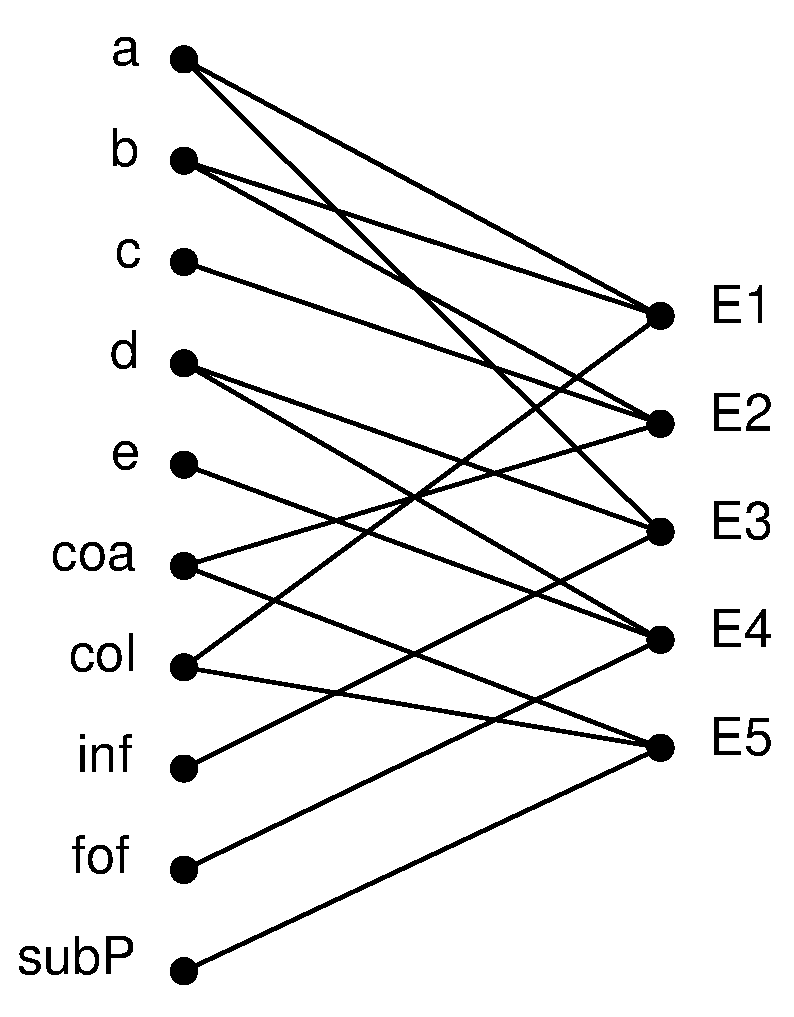
\includegraphics[width=.7\textwidth]{fig/BG-black.eps}
\end{minipage}
\caption[An example incidence matrix of a hypergraph]{\label{fig:incidence}Incidence matrix representing the hypergraph of figure~\ref{fig:graphcomp}(B) and the corresponding incidence graph.}
\end{figure}

RDF bipartite graphs have many desirable properties for developing intuitive mining algorithms because they turn hypergraphs into a simple form so that many algorithms designed on simple graphs can be readily applied. Therefore, we propose to use bipartite graphs to represent domain knowledge and data expressed in RDF.

\begin{myexp}[\textbf{Hypergraph incidence matrix and corresponding bipartite graph}]
\label{incidence}
Figure~\ref{fig:incidence} (A) shows the incidence matrix according to the hypergraph in Figure~\ref{fig:graphcomp} from Example~\ref{ex:inconsistentDG}. And Figure~\ref{fig:incidence} (B) shows the corresponding bipartite graph. Hypergraph incidence matrices represent membership of a node in an edge with a ``1" in the corresponding entry.
\end{myexp}

Example~\ref{incidence} illustrates the general method that can be applied to all hypergraphs to transform to their bipartite graph form. In the case of a hypergraph representing an RDF graph, since nodes in an RDF statement are ordered (subject followed by predicate then object), this ordering must be preserved in the incidence matrix. A \emph{labeled bipartite graph} can be derived to further capture the ordering and roles of nodes.

\begin{mydef}[\textbf{RDF labeled bipartite graph}]
In the hypergraph incidence matrix, instead of using ``1/0'' according to the occurrence of a node in a hyperedge, we choose to label them by S, P or O to represent the role (subject, predicate, or object) of the node from the underlying RDF statement. Hence, when deriving the bipartite graph of a hypergraph incidence matrix, an edge is added for every S, P, O entry of the matrix, and this edge will be labeled with a corresponding character (S, P, or O). Thus, the only difference between the graph derived from the incidence matrix of any hypergraph and an RDF hypergraph is the fact that each edge has one out of three labels~\cite{GraphModelRDF}.
\end{mydef}

In the rest of the dissertation, when we use the term RDF bipartite graph, we mean RDF labeled bipartite graph for short.

\begin{myexp}[\textbf{RDF labeled bipartite graph}]
Figure~\ref{fig:graphcomp-bio} illustrates an example of RDF hypergraph represented as labeled bipartite graph. The left side shows a portion of an ontology in biomedical domain on zebrafish anatomy~\cite{ZFA} visualized as a directed labeled graph. Two different relationships are depicted in the figure, namely, ``subClassOf" and ``part\_of." The corresponding labeled bipartite graph representation is shown on the right side. Circle nodes are \emph{statement nodes} representing RDF statements. Each statement node is connected to three \emph{value nodes} representing three components of a statement (subject, predicate, and object). Edge labels S, P, and O indicate the role of the value nodes in the statement.
\end{myexp}

\begin{figure}[tbh]
\centering
\begin{minipage}[c]{0.35\textwidth}\flushright
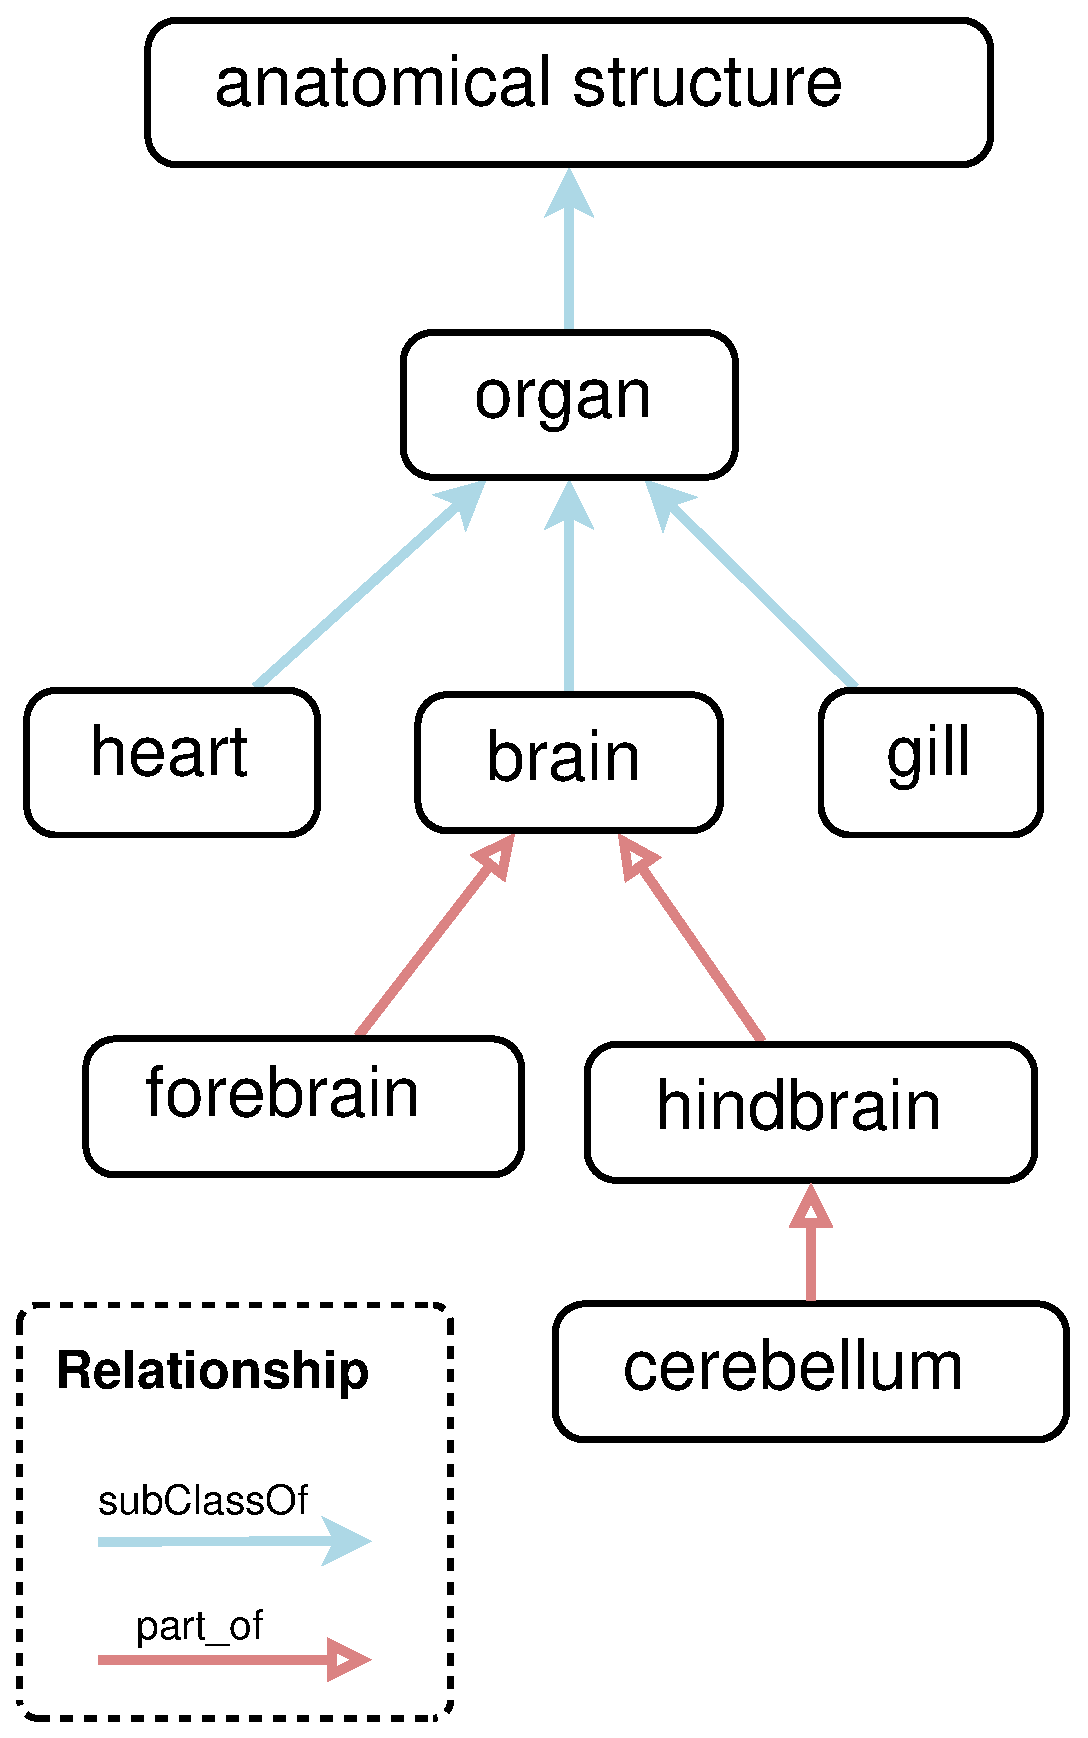
\includegraphics[width=.7\textwidth]{fig/DLG-bio.eps}
\end{minipage}\hfill
\begin{minipage}[c]{0.6\textwidth}\centering
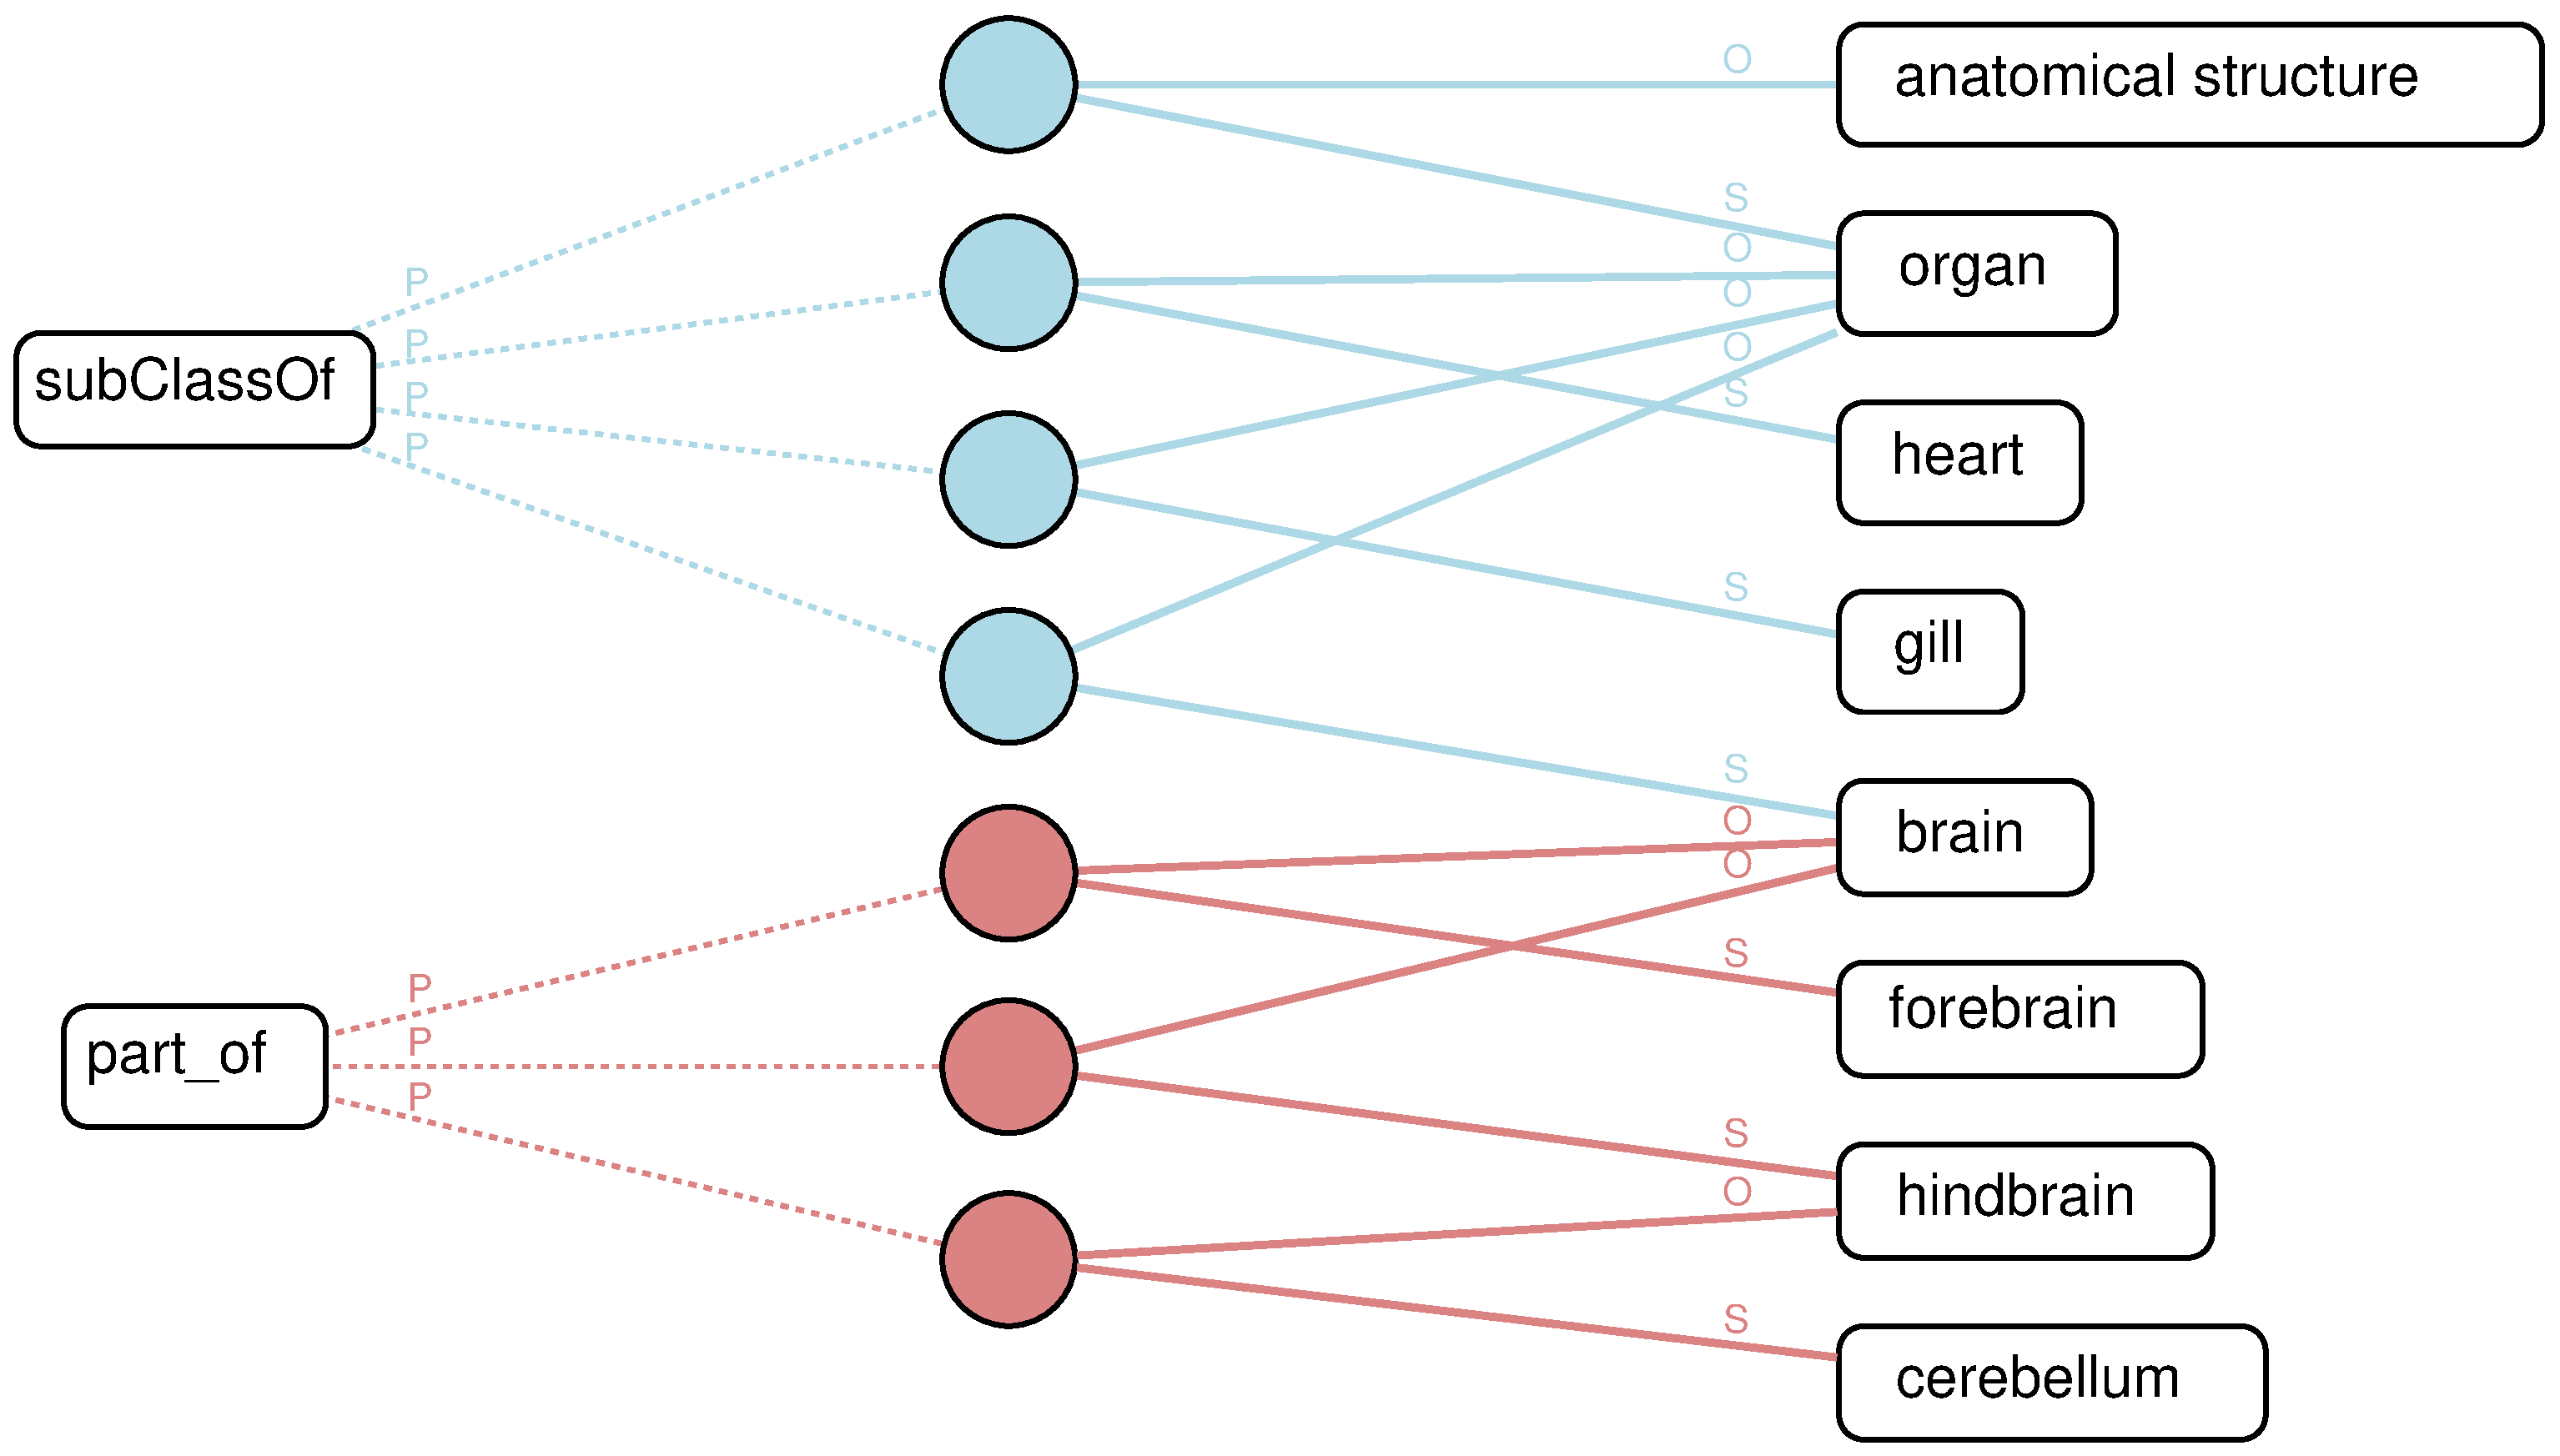
\includegraphics[width=\textwidth]{fig/BG-bio.eps}\\
\end{minipage}
\caption[A comparison between the directed labeled graph and the RDF bipartite graph]{\label{fig:graphcomp-bio} A portion of a zebrafish anatomy ontology represented as a directed labeled graph (A) and an RDF bipartite graph (B)}
\end{figure}

\section{Graph Representation for Relational Structures}
\label{sec:graph-rep-for-rdb}
Various graph representations for relational structures have been proposed in the literature to tackle different data mining tasks. For example, in the case of frequent itemset mining, a set of objects with co-occurrence relationships can be represented as directed or undirected graphs (see the example in Figure~\ref{fig:hg_and_rg}, Chapter~\ref{chap:background}).

Another way to represent a relational structure is to first transform it to RDF, and given the graph nature of RDF, the relational structure can then be represented as a graph. Mapping from an RDB (relational database) to RDF has gained increasing attention and led to the implementation of generic mapping tools as well as domain--specific applications.  The W3C launched the RDB2RDF incubator group to explore issues involved in mapping RDB to RDF. A work-in-progress survey paper has been published documenting approaches in this field~\cite{RDB2RDF}.

%We can classify the methods used to generate the mappings between RDB and RDF into two categories:
A straightforward method for mapping an RDB to RDF is discussed by Berners-Lee~\cite{TBL98} as defined in the following.

\begin{mydef}[\textbf{Context--independent mapping from an RDB to RDF}]
Without linking to any explicit definition of domain semantics (such as those defined in domain ontologies), an RDB can be transformed to RDF following the steps below:
\begin{enumerate}
\label{auto-map}
\item An RDB row is an RDF subject node.
\item A column of an RDB table is a predicate node.
\item A cell value of an RDB table is an object node.
\end{enumerate}
\end{mydef}

Many systems leverage these mappings to automatically generate mappings from an RDB to RDF. Even though these automatically generated mappings often do not capture complex domain semantics that are required by many applications, these mappings can be used as a starting point to create more customized, domain--specific mappings.

\begin{myexp}[\textbf{RDF bipartite graph for a nominal-valued RDB}]
Table~\ref{tbl:nominal-rel} (A) shows a relational table with nominal features. The table has $m$ rows, annotated by labels $r_1 \ldots r_m$, and $n$ columns named $f_1 \ldots f_n$. Applying the steps in Definition~\ref{auto-map} for mapping an RDB to RDF mapping, the corresponding RDF statements are listed in Table~\ref{tbl:nominal-rel} (B). From these statements, an RDF bipartite graph is derived, (see Figure~\ref{fig:BG-relational-nominal}), as the graph representation for the underlying relational table in Table~\ref{tbl:nominal-rel} (A).
\end{myexp}

\begin{table}[ht]
\begin{minipage}[c]{0.4\linewidth}\begin{flushright}
\begin{tabular}{ c | c | c | c |}
\cline{2-4}
	~   & $f_1$	    & $\cdots$  & $f_n$   \\
\cline{2-4}
$r_1:$	& $v_{11}$	& $\cdots$  & $v_{1n}$\\
\cline{2-4}
$\vdots$& $\vdots$  & $\ddots$  & $\vdots$\\
\cline{2-4}
$r_m:$	& $v_{m1}$	& $\cdots$  & $v_{mn}$\\
\cline{2-4}
\end{tabular}
\end{flushright}
\end{minipage}
\hfill
\begin{minipage}[c]{0.4\linewidth}
\begin{tabular}{c c c}
\emph{s}&   \emph{p}&  \emph{o}\\
\texttt{<$r_1$>}   &  \texttt{<$f_1$>}  &  \texttt{<$v_{11}$>}\\
\texttt{<$r_1$>}   &  \texttt{<$f_n$>}  &  \texttt{<$v_{1n}$>}\\
\texttt{<$r_m$>}   &  \texttt{<$f_1$>}  &  \texttt{<$v_{m1}$>}\\
\texttt{<$r_m$>}   &  \texttt{<$f_n$>}  &  \texttt{<$v_{mn}$>}\\
\end{tabular}
\end{minipage}
\begin{minipage}[c]{0.4\linewidth}\centering
\vspace{0.2cm}\hspace{2.8cm}(A)
\end{minipage}
\begin{minipage}[c]{0.4\linewidth}\centering
\vspace{0.2cm}\hspace{3.5cm}(B)
\end{minipage}
\caption[An example relational table with nominal features and the corresponding RDF]{\label{tbl:nominal-rel} An example of a relational table with nominal features (A) and its corresponding RDF triple form (B).}
\end{table}

\begin{figure}[tbh]
\begin{center}
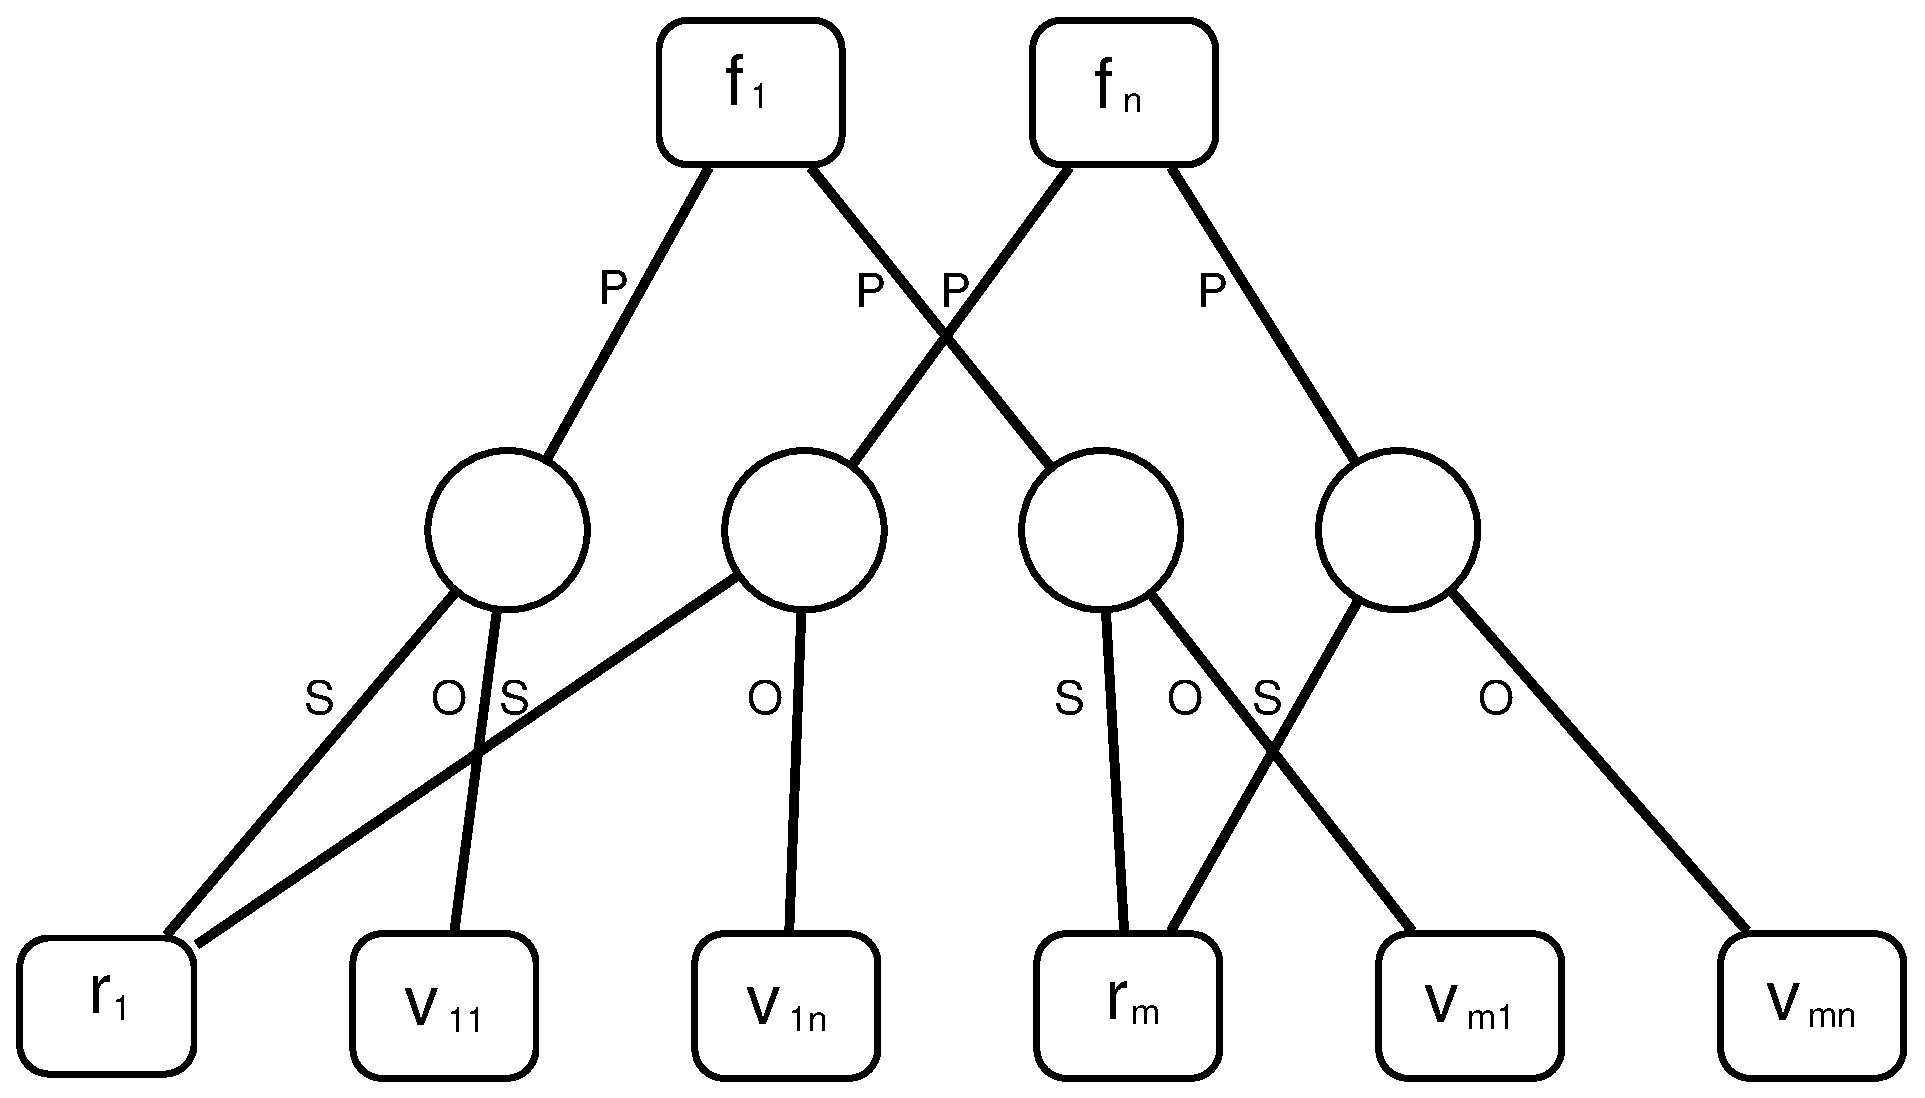
\includegraphics[width=.5\textwidth]{fig/BG-relational-nominal.eps}
\end{center}
\caption[The RDF bipartite graph for a nominal-valued table]{\label{fig:BG-relational-nominal} An RDF bipartite graph based on RDF triples in Table~\ref{tbl:nominal-rel} (B).}
\end{figure}

For relational tables with binary (Boolean) features, the RDF representation can be more compact. In some applications, only cells with positive (``1") values are of interest. In such case, an auxiliary predicate can be introduced to link a row with positive cell values in that row. Example~\ref{exp:repBinRDB} illustrates this point.

\begin{myexp}[\textbf{RDF bipartite graph from positive values of a binary-valued RDB}]
\label{exp:repBinRDB}
Table~\ref{tbl:binary-rel} (A) shows an $m$-by-$n$ relational table with binary features. We use an auxiliary predicate \texttt{<mentions>} to denote a positive occurrence of a feature in one row. For example, the statement \texttt{<$r_1$> <mentions> <$f_n$>} corresponds to the value ``1" in the $n$-th feature in the first row. Consequently, the whole Table~\ref{tbl:binary-rel} (A) maps to only two RDF statements in Table~\ref{tbl:binary-rel} (B).
\end{myexp}


\begin{table}[ht]
\begin{minipage}[b]{0.38\linewidth}\begin{flushright}
\begin{tabular}{ c | c | c | c |}
\cline{2-4}
	~   & $f_1$	    & $\cdots$  & $f_n$   \\
\cline{2-4}
$r_1:$	&  0  	& $\cdots$   &    1  \\
\cline{2-4}
$\vdots$& $\vdots$  & $\ddots$  & $\vdots$\\
\cline{2-4}
$r_m:$	&  1  	& $\cdots$   &    0  \\
\cline{2-4}
\end{tabular}
\end{flushright}
\end{minipage}
\hfill
\begin{minipage}[b]{0.4\linewidth}
\begin{tabular}{c c c}
\emph{s}&   \emph{p}&  \emph{o}\\
\texttt{<$r_1$>}   &    \texttt{<mentions>}   &  \texttt{<$f_n$>}\\
\texttt{<$r_m$>}   &    \texttt{<mentions>}   &  \texttt{<$f_1$>}\\
\end{tabular}
\end{minipage}
\begin{minipage}[c]{0.4\linewidth}\centering
\vspace{0.2cm}\hspace{2.8cm}(A)
\end{minipage}
\begin{minipage}[c]{0.4\linewidth}\centering
\vspace{0.2cm}\hspace{3.5cm}(B)
\end{minipage}
\caption{\label{tbl:binary-rel} An example relational table with binary features.}
\end{table}

Using the auxiliary predicate (\texttt{<mentions>}) greatly simplifies the resulting RDF graph by reducing the number of distinct predicates from $n$, according to the process in Definition~\ref{auto-map}, to only 1. This has profound implications for developing efficient analysis and mining methods based on the RDF bipartite graph.

However, the auxiliary predicate is feasible only when linking a row node with its positive value nodes in a binary-valued scenario. If negative cell values are also of interest and need to be included, the trick shown in the following example can be performed so that we can still use a single auxiliary predicate.

\begin{myexp}[\textbf{RDF bipartite graph from both positive and negative values of a binary-valued RDB}]
\label{binary-reverse}
Table~\ref{tbl:binary-rel-expansion} (A) is derived from Table~\ref{tbl:binary-rel} (A) by adding a reverse column for each of its original columns: For each $f_i$, $i \in [1, n]$, a reverse $f_i'$ is created so that feature values $v_{ki} = \neg v_{ki'}$,  $\forall{k\in[1,m]}$. In this way, we can use the auxiliary predicate \texttt{<mentions>} to link to negative values by using the reverse column, because, for example, \texttt{<$r_1$> <mentions> <$f_1'$>} is equivalent to \texttt{<$r_1$> <mentions> $\neg$<$f_1$>}~. Table~\ref{tbl:binary-rel-expansion} (B) shows the RDF statements based on Table~\ref{tbl:binary-rel-expansion} (A) which essentially captures information of both positive and negative values from Table~\ref{tbl:binary-rel} (A).
\end{myexp}

\begin{table}[ht]
\begin{minipage}[b]{0.4\linewidth}\begin{flushright}
\begin{tabular}{ c | c | c | c | c | c |}
\cline{2-6}
	~   & $f_1$	 &  $f_1'$  & $\cdots$  & $f_n$  &  $f_n'$ \\
\cline{2-6}
$r_1:$	&  0  &  1	& $\cdots$   &    1  & 0\\
\cline{2-6}
$\vdots$& $\vdots$ & $\vdots$  & $\ddots$  & $\vdots$ & $\vdots$\\
\cline{2-6}
$r_m:$	&  1  &  0	& $\cdots$   &    0  & 1\\
\cline{2-6}
\end{tabular}
\end{flushright}
\end{minipage}
\hfill
\begin{minipage}[b]{0.4\linewidth}
\begin{tabular}{c c c}
\emph{s}&   \emph{p}&  \emph{o}\\
\texttt{<$r_1$>}   &    \texttt{<mentions>}   &  \texttt{<$f_1'$>}\\
\texttt{<$r_1$>}   &    \texttt{<mentions>}   &  \texttt{<$f_n$>}\\
\texttt{<$r_m$>}   &    \texttt{<mentions>}   &  \texttt{<$f_1$>}\\
\texttt{<$r_m$>}   &    \texttt{<mentions>}   &  \texttt{<$f_n'$>}\\
\end{tabular}
\end{minipage}
\hspace{1.5cm}
\begin{minipage}[c]{0.4\linewidth}\centering
\vspace{0.2cm}\hspace{2.8cm}(A)
\end{minipage}
\begin{minipage}[c]{0.4\linewidth}\centering
\vspace{0.2cm}\hspace{3.5cm}(B)
\end{minipage}
\caption{\label{tbl:binary-rel-expansion} An example expanded relational table with binary features.}
\end{table}

The process of adding reverse columns to binary-valued RDB tables described in Example~\ref{binary-reverse} can be extended to nominal-valued tables as well. By doing this we can achieve the desirable property of having only one predicate in the resulting RDF representation. The process is called RDB nominal value expansion as defined below.

\begin{mydef}[\textbf{RDB nominal value expansion}]
\label{nominal-expansion}
In a nominal valued RDB table, for each feature $f_i$ taking values on the set $V_i=\{v_{i1}, v_{i2}, \ldots\}$, we denote $|V_i|$ as the number of distinct values of $f_i$. The RDB nominal value expansion is the process to transform each nominal feature $f_i$ to $|V_i|$ number of binary features ($f_{i1}, f_{i2}, \ldots, f_{i|V_i|}$). The value of $k$-th row in $f_{ij}, (j\in [1, |V_i|)$, is ``1", if and only if $f_i$ takes the value $v_{ij}$ in the $k$-th row.
\end{mydef}

\begin{myexp}[\textbf{RDB nominal value expansion}]
Table~\ref{tbl:nominal-rel-expansion} (A) shows a nominal-valued RDB table with meaningful column names and values. We use the notation, Outlook=\{sunny, overcast, rainy\}, to denote the set of distinct values the feature ``Outlook" can take on. Similarly, we have Temperature=\{hot, mild, cool\}, and Humidity=\{high, low\}. Table~\ref{tbl:nominal-rel-expansion} (B) shows the resulting table after nominal value expansion based on Definition~\ref{nominal-expansion}. RDF statements are then derived using one single auxiliary predicate \texttt{<mentions>}, as partly shown in Table~\ref{tbl:nominal-rel-expansion} (C).
\end{myexp}

\begin{table}[ht]
\begin{minipage}[b]{0.35\linewidth}
\begin{tabular}{ c | c | c | c |}
\cline{2-4}
	~   & O	    & T  & H   \\
\cline{2-4}
$r_1:$	&    sunny & hot & high  \\
\cline{2-4}
$r_2$:  &   rainy  & cool  & low\\
\cline{2-4}
$\vdots$& \multicolumn{3}{c|}{$\vdots$}\\
\cline{2-4}
$r_m:$	&  overcast  	& mild   & low  \\
\cline{2-4}
\end{tabular}
\end{minipage}
\begin{minipage}[b]{0.55\linewidth}
\begin{tabular}{ c | c | c | c || c | c | c || c | c |}
\cline{2-9}
~     & O\_s & O\_o & O\_r & T\_h & T\_m & T\_c & H\_h & H\_l \\
\cline{2-9}
$r_1:$ & 1 & 0 & 0 & 1 & 0 & 0 & 1 & 0 \\
\cline{2-9}
$r_2:$ & 0 & 0 & 1 & 0 & 0 & 1 & 0 & 1 \\
\cline{2-9}
$\vdots$& \multicolumn{8}{c|}{$\vdots$}\\
\cline{2-9}
$r_m:$ & 0 & 1 & 0 & 0 & 1 & 0 & 0 & 1 \\
\cline{2-9}
\end{tabular}
\end{minipage}
\hspace{1.5cm}
\begin{minipage}[c]{0.35\linewidth}\centering
\vspace{0.2cm}\hspace{1.5cm}(A)
\end{minipage}
\begin{minipage}[c]{0.55\linewidth}\centering
\vspace{0.2cm}\hspace{1.5cm}(B)
\end{minipage}
\begin{minipage}[b]{\linewidth}\centering
\begin{tabular}{c c c}
&&\\
\emph{s}&   \emph{p}&  \emph{o}\\
\texttt{<$r_1$>}   &    \texttt{<mentions>}   &  \texttt{<O\_s>}\\
\texttt{<$r_1$>}   &    \texttt{<mentions>}   &  \texttt{<T\_h>}\\
\texttt{<$r_1$>}   &    \texttt{<mentions>}   &  \texttt{<H\_h>}\\
\texttt{<$r_2$>}   &    \texttt{<mentions>}   &  \texttt{<O\_r>}\\
\multicolumn{3}{c}{$\cdots$}\\
\multicolumn{3}{c}{(C)}\\
\end{tabular}
\end{minipage}
\caption[Nominal value expansion for a relational table and the resulting RDF triples.]{\label{tbl:nominal-rel-expansion} An example nominal-valued relational table after nominal value expansion. (A) shows the original table where O stands for ``outlook," T for ``temperature" and "H" for humidity. (B) shows the expanded table. (C) shows the corresponding RDF triples derived from (B).}
\end{table}

\section{Combining Data Graphs and Ontology Graphs}

In order to facilitate the synergy between data and domain knowledge in a mining framework, information from both sources needs to be first combined. This is achieved by the process called \emph{semantic annotation}. Semantic annotation aims at assigning formal semantic descriptions to the basic element of data, and it is crucial in realizing semantic data mining by bridging formal semantics in domain knowledge with data. A number of previous research efforts have been devoted to this direction, resulting in various methodologies and systems, such as the NCBO (National Center of Biomedical Ontology) annotator~\cite{RI} that generates the electronic health dataset for our experiments described in Chapter~\ref{chap:datamining} and~\ref{chap:miningWithOnto}. Also, readers are referred to Reeve and Han~\cite{Reeve2005SurveyAnnotation} for a general survey on semantic annotation.

In the following, we assume data is annotated, meaning that links from entities in data to formal semantic descriptions (such as those in ontologies) are already established. A unified graph incorporating information from both data and ontologies can be created. Data mining algorithms dealing with such unified graph representation can enjoy the benefit of a seamless integration of domain knowledge. The following example shows the combination of an ontology graph and a data graph.

%\textbf{b) Domain Semantics--driven Mapping Generation}: The second approach generates mappings from RDB to RDF by incorporating domain semantics that is often implicit or not captured at all in the RDB schema. The explicit modeling of domain semantics, often modeled as a domain ontology. The domain ontology may be pre--existing and sourced from public resources.

\begin{myexp}[\textbf{Combining an ontology graph and a data graph}]
\label{exp:combineRdfBipartite}
Figure~\ref{fig:onto-and-data} (A) shows a simple ontology in a certain domain with only subsumption relationships defined for five concepts (A--B). Figure~\ref{fig:onto-and-data} (B) shows a binary-valued RDB table in the same domain with the set of concepts (A--B) being features. We use the same concept labels in the ontology and the RDB table because we assume the mapping between the ontology nodes and the table features are pre-assigned manually or established by automatic annotation. Figure~\ref{fig:hypergraph-combined} (B) shows the RDF statements derived from both the ontology and the RDB table. Figure~\ref{fig:hypergraph-combined} (A) demonstrates the combined RDF bipartite graph.

Nodes in Figure~\ref{fig:hypergraph-combined} (A) can be rearranged to a particular form as shown Figure~\ref{fig:bipartitegraph-weighted}. This graph demonstrates a tripartite structure where row nodes ($r_1$--$r_5$) fall on one partition, column nodes (A--E) on another, and statement nodes in between. A plethora of graph mining techniques can be leveraged to analyze the path configuration in this graph to answer interesting questions such as the grouping of rows and columns (\eg, to solve the the task of clustering and association mining respectively). Predicate nodes can serve as hints to introduce different weights to paths in order to distinguish different semantic types and capture their relative strengths.

Edge and statement nodes in Figure~\ref{fig:bipartitegraph-weighted} are depicted in two colors to signify their sources of origin. Red edges and nodes denote information from data (RDB table), and blue ones from the ontology. We notice from the graph that the contribution of the ontology can be viewed as to introduce extra paths of different semantic types (The data is structured under the ``mentions" relationship and the ontology is structured under the subsumption relationship). In this way, a data mining algorithm that is able to deal with the data graph can be naturally extended without major modifications to handle domain knowledge coded in the ontology.
\end{myexp}

\begin{figure}[tbh]
\begin{minipage}[c]{.45\textwidth}\centering
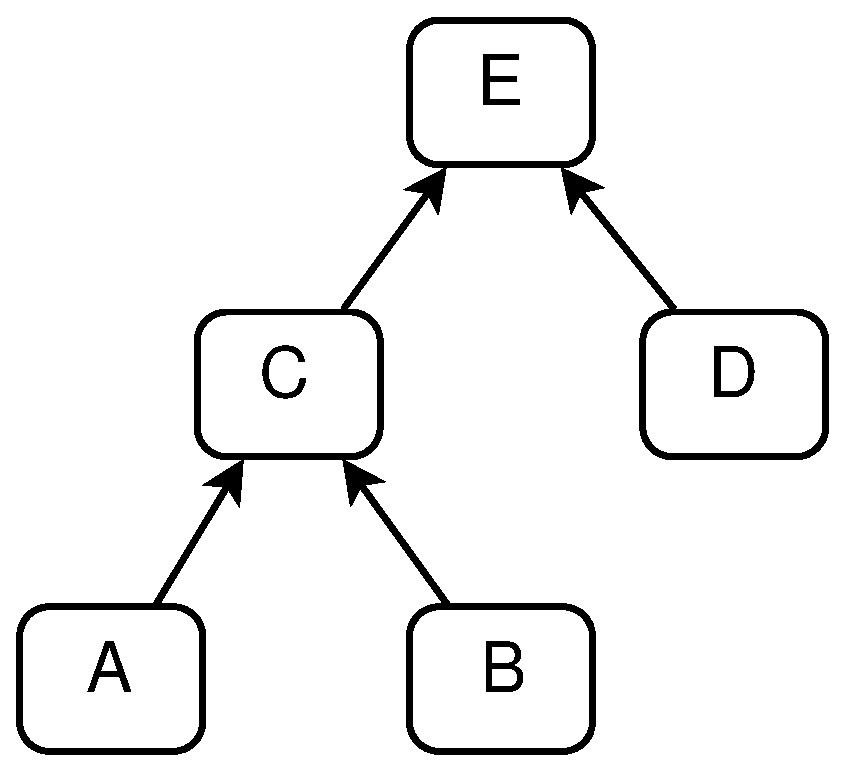
\includegraphics[width=.5\linewidth]{fig/simple-onto.eps}
\end{minipage}
\begin{minipage}[b]{.45\textwidth}\centering
    \begin{tabular}{ c | c | c | c | c | c |}
    \cline{2-6}
    	~ & A & B & C & D & E\\
    \cline{2-6}
    $r_1:$& 1 & 1 & 0 & 0 & 0 \\
    \cline{2-6}
    $r_2:$& 1 & 1 & 1 & 0 & 0 \\
    \cline{2-6}
    $r_3:$& 0 & 1 & 1 & 0 & 0 \\
    \cline{2-6}
    $r_3:$& 0 & 0 & 0 & 1 & 0 \\
    \cline{2-6}
    \end{tabular}
\end{minipage}
\begin{minipage}[c]{0.4\linewidth}\centering
\vspace{0.2cm}\hspace{2cm}(A)
\end{minipage}
\begin{minipage}[c]{0.4\linewidth}\centering
\vspace{0.2cm}\hspace{4cm}(B)
\end{minipage}
\caption[An example relational table and a domain ontology]{\label{fig:onto-and-data} An example of a binary-valued relational table (B) about five concepts (``A"--``E"), and the ontological relationship among these concepts shown as a directed graph (A).}
\end{figure}

\begin{figure}[tbh]
\begin{center}
\begin{tabular}{c  c}
\multirow{12}{*}{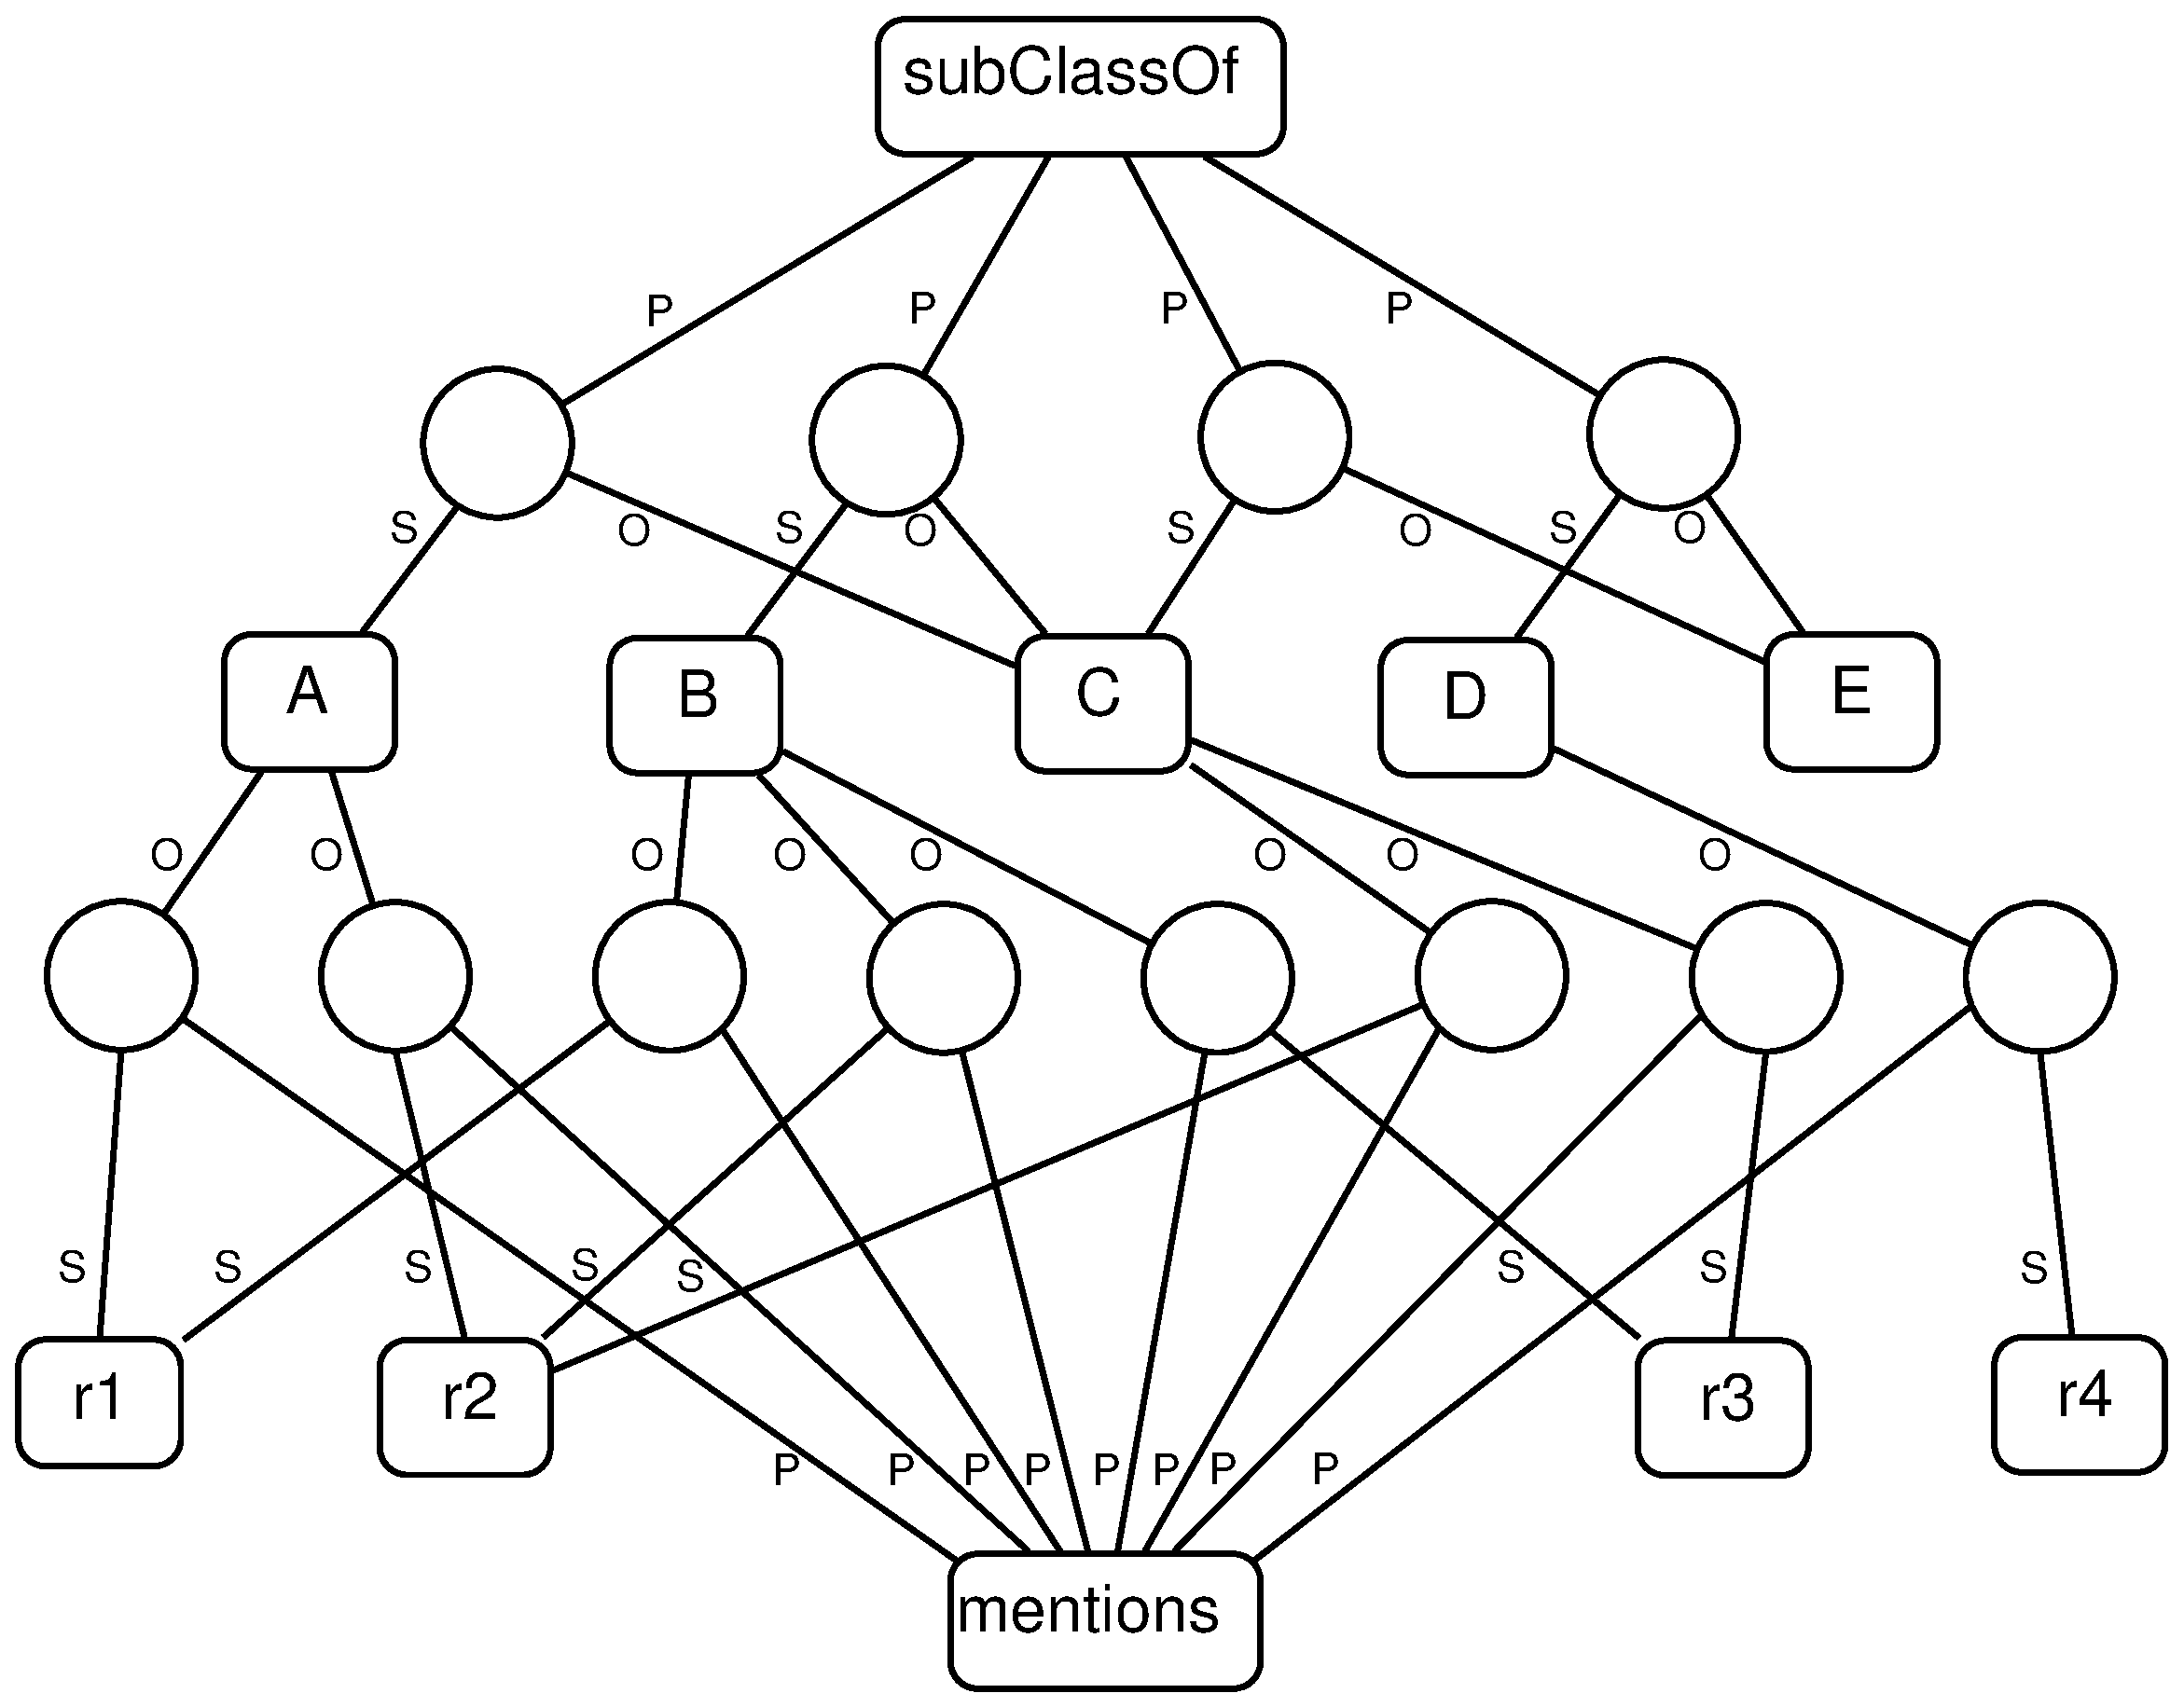
\includegraphics[width=.55\textwidth]{fig/hypergraph_mining.eps}} & \emph{~~~s \hfill p\hfill o~~~}\\
& \texttt{<A>~~<subClassOf>~~<C>}\\
& \texttt{<B>~~<subClassOf>~~<C>}\\
& \texttt{<C>~~<subClassOf>~~<E>}\\
& \texttt{<D>~~<subClassOf>~~<E>}\\
& \\
& \texttt{<r1>\;~~<mentions>\;~~<A>}\\
& \texttt{<r1>\;~~<mentions>\;~~<B>}\\
& \texttt{<r2>\;~~<mentions>\;~~<A>}\\
& \texttt{<r2>\;~~<mentions>\;~~<B>}\\
& \texttt{<r2>\;~~<mentions>\;~~<C>}\\
& \texttt{<r3>\;~~<mentions>\;~~<B>}\\
& \texttt{<r3>\;~~<mentions>\;~~<C>}\\
& \texttt{<r4>\;~~<mentions>\;~~<D>}\\
& \\
& \\
(A) & (B)\\
\end{tabular}
\end{center}
\caption[The RDF bipartite graph as the combined representation]{\label{fig:hypergraph-combined} The RDF bipartite graph representation (A) given triples shown in (B) based on the information described in Figure~\ref{fig:onto-and-data}.}
\end{figure}

\begin{figure}[tbh]
\begin{center}
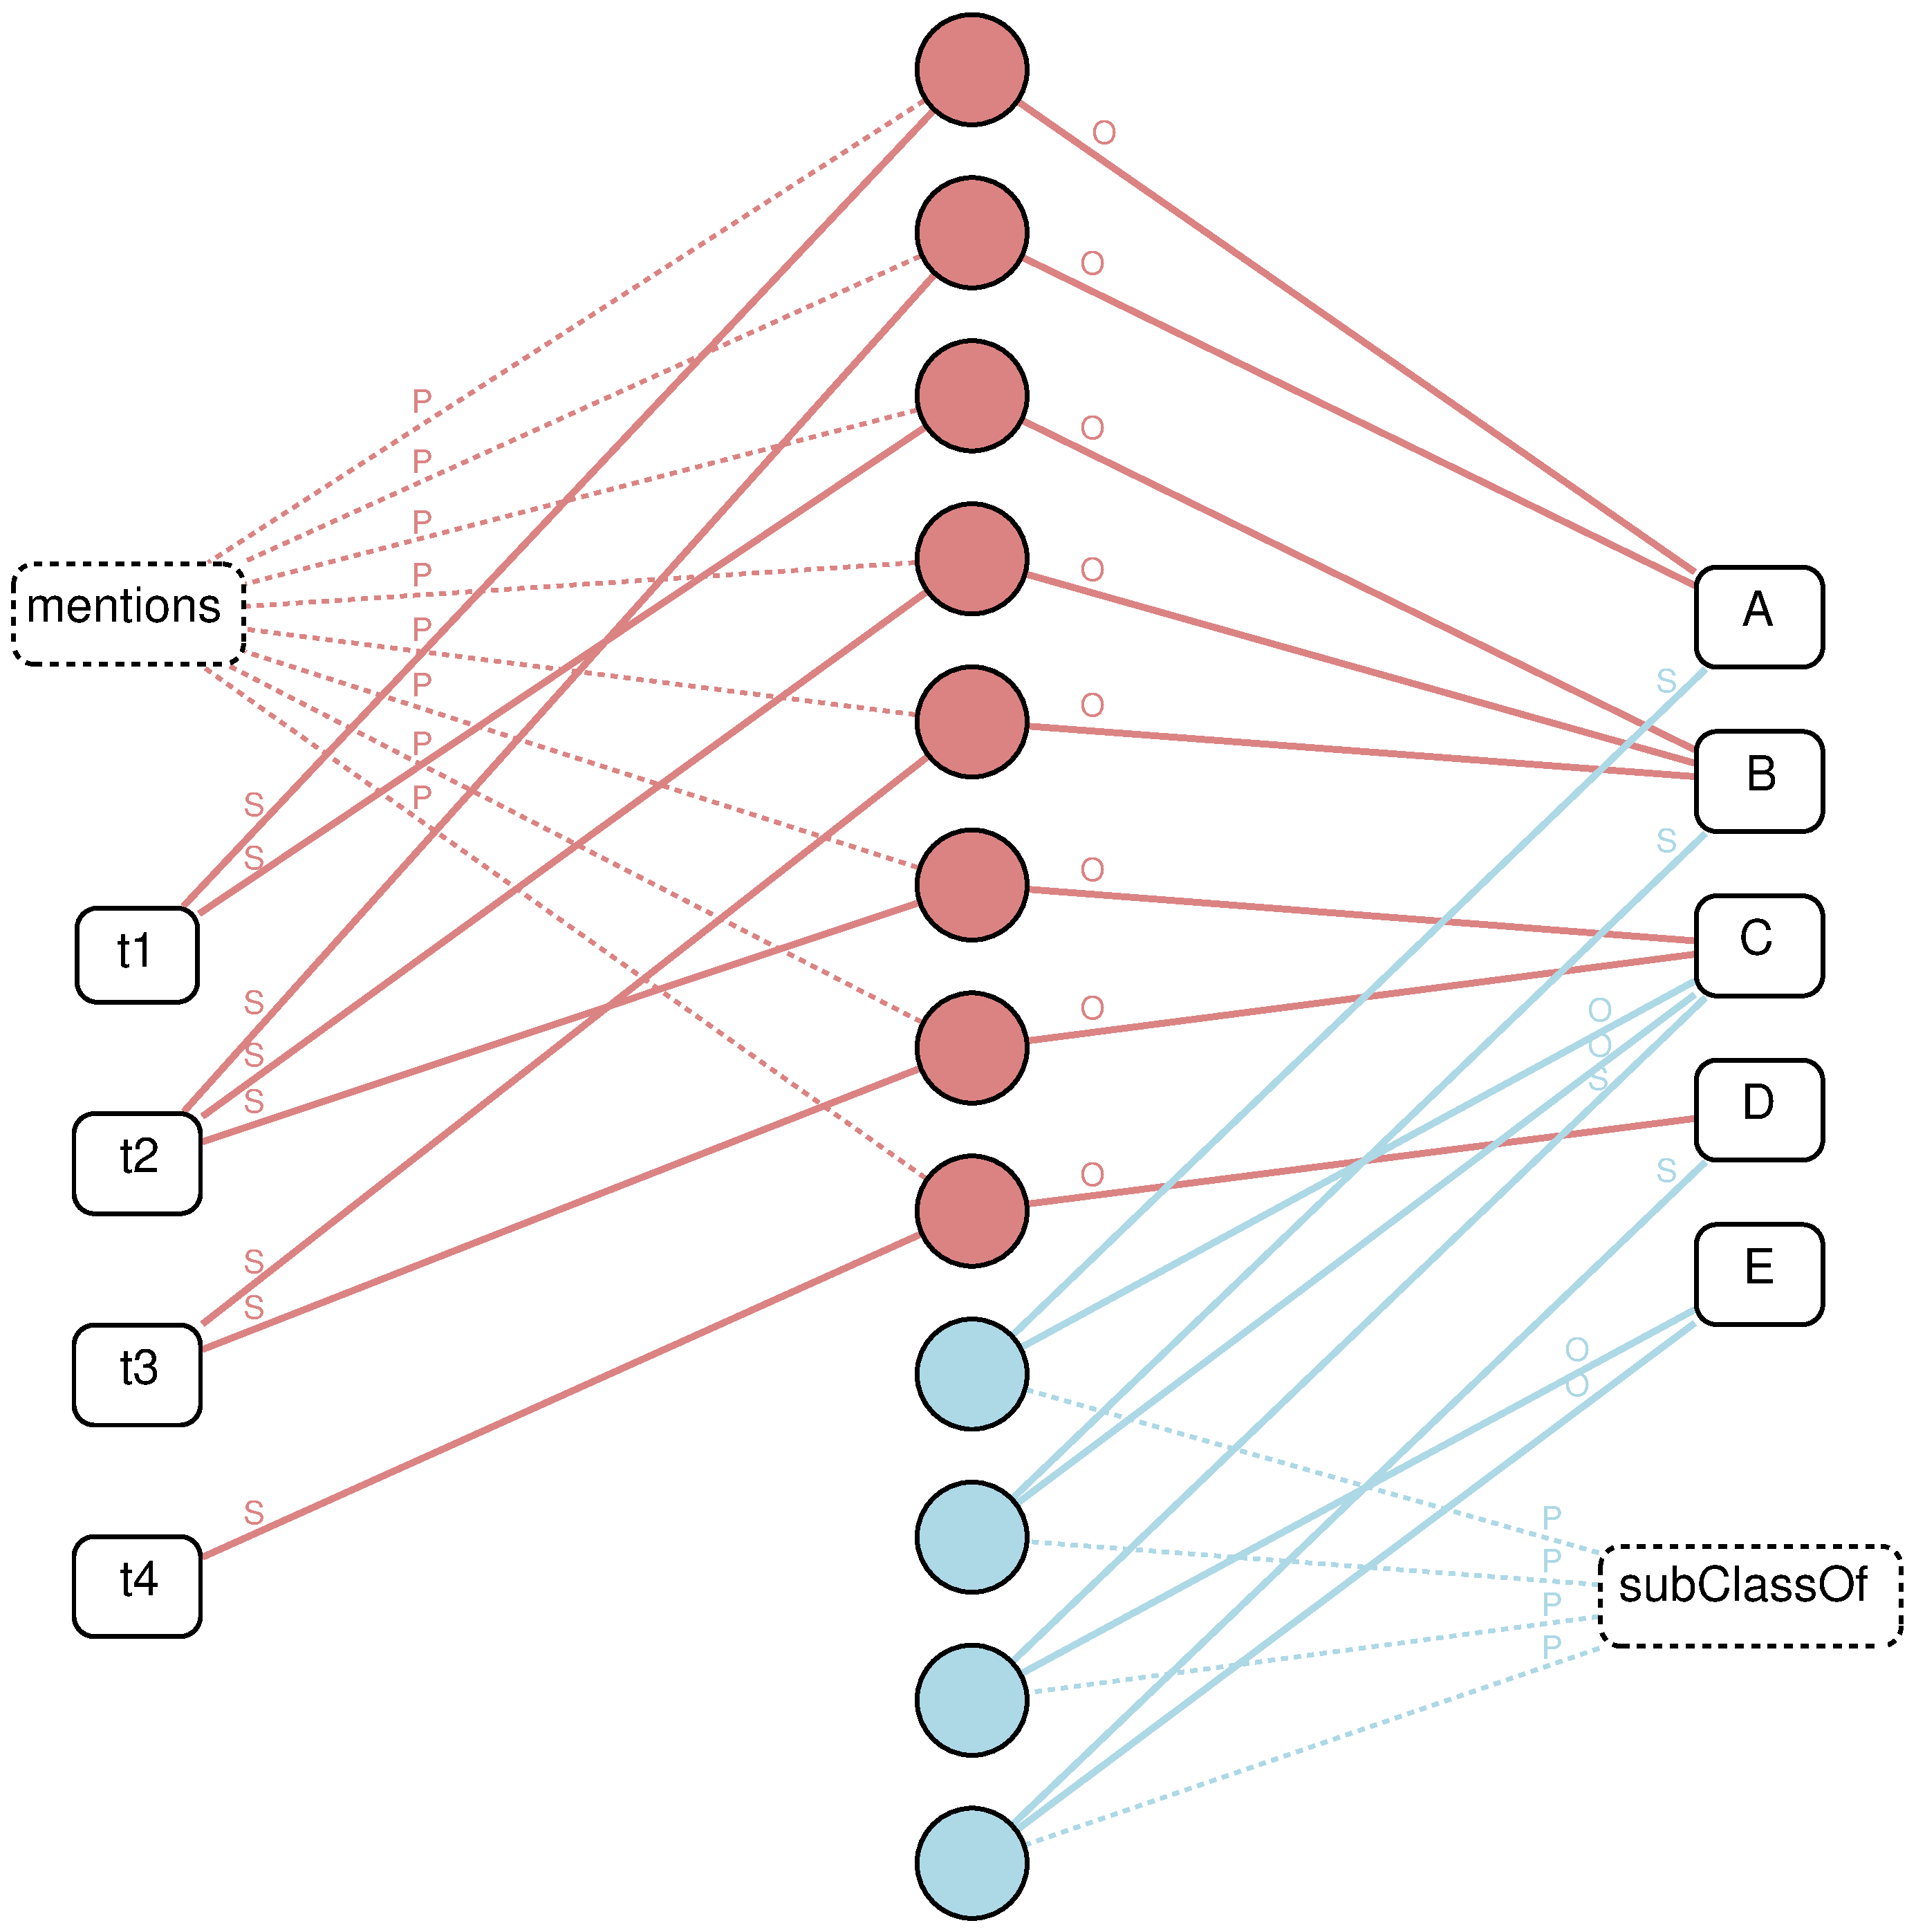
\includegraphics[width=.5\textwidth]{fig/hypergraph_mining-bipartite-weighted.eps}
\end{center}
\caption[Transforming the RDF bipartite graph to suit mining need]{\label{fig:bipartitegraph-weighted} This figure shows that, grouping the nodes according to whether they are row elements or column elements in Figure~\ref{fig:onto-and-data} (B), the bipartite graph shown in Figure~\ref{fig:hypergraph-combined} (A) can be further transformed to a tripartite graph.}
\end{figure}

\subsection{Representing Different Kinds of Ontological Semantics}
\label{sec:rosg}

%In our preliminary work, we have showed a way to represent ontology annotated data in hypergraphs which help discovering semantic associations.  If the domain knowledge is defined as formal ontologies, it is a natural thinking to use graphs to represent the domain knowledge as well. To formally represent domain knowledge using graphs, it is important to different types of formal semantics in a systematic way.

In order to leverage the increasingly larger and richer collection of domain ontologies, especially in scientific fields such as the biomedical domain, we propose to use weights to distinguish paths in the RDF bipartite graph representing different semantic types or relationships (properties) from the ontology, such as class subsumption, part\_of, and other general or domain--specific properties. The weights also characterize the relative importance of the paths. %(e.g., Drug \textit{treat} Disease).

\begin{myexp}[\textbf{Assigning weights to different relationship}]
Figure~\ref{fig:hypergraph_mining-comp} shows an example of an RDF bipartite graph representing information about a group of people (A--E) where multiple relationships can be identified among them. For example, A, B, C and D are linked by the coauthorship relationship, while D and E are linked by the more general collaboration relationship (in fact, coauthorship is defined as a sub-property of collaboration in the ontology). A, B and C are professors, D and E are PhD students, and both professors and PhD students are researchers. In this complex network of relationships, we can distinguish their roles and importance by assigning application--specific weights to the related paths (\eg, different colorings in the graph denotes different weights assigned to the paths). %In order to achieve this, we propose to develop a framework for guiding the (semi-) automatic assignment of weights.
\end{myexp}

\begin{figure}[tbh]
\begin{center}
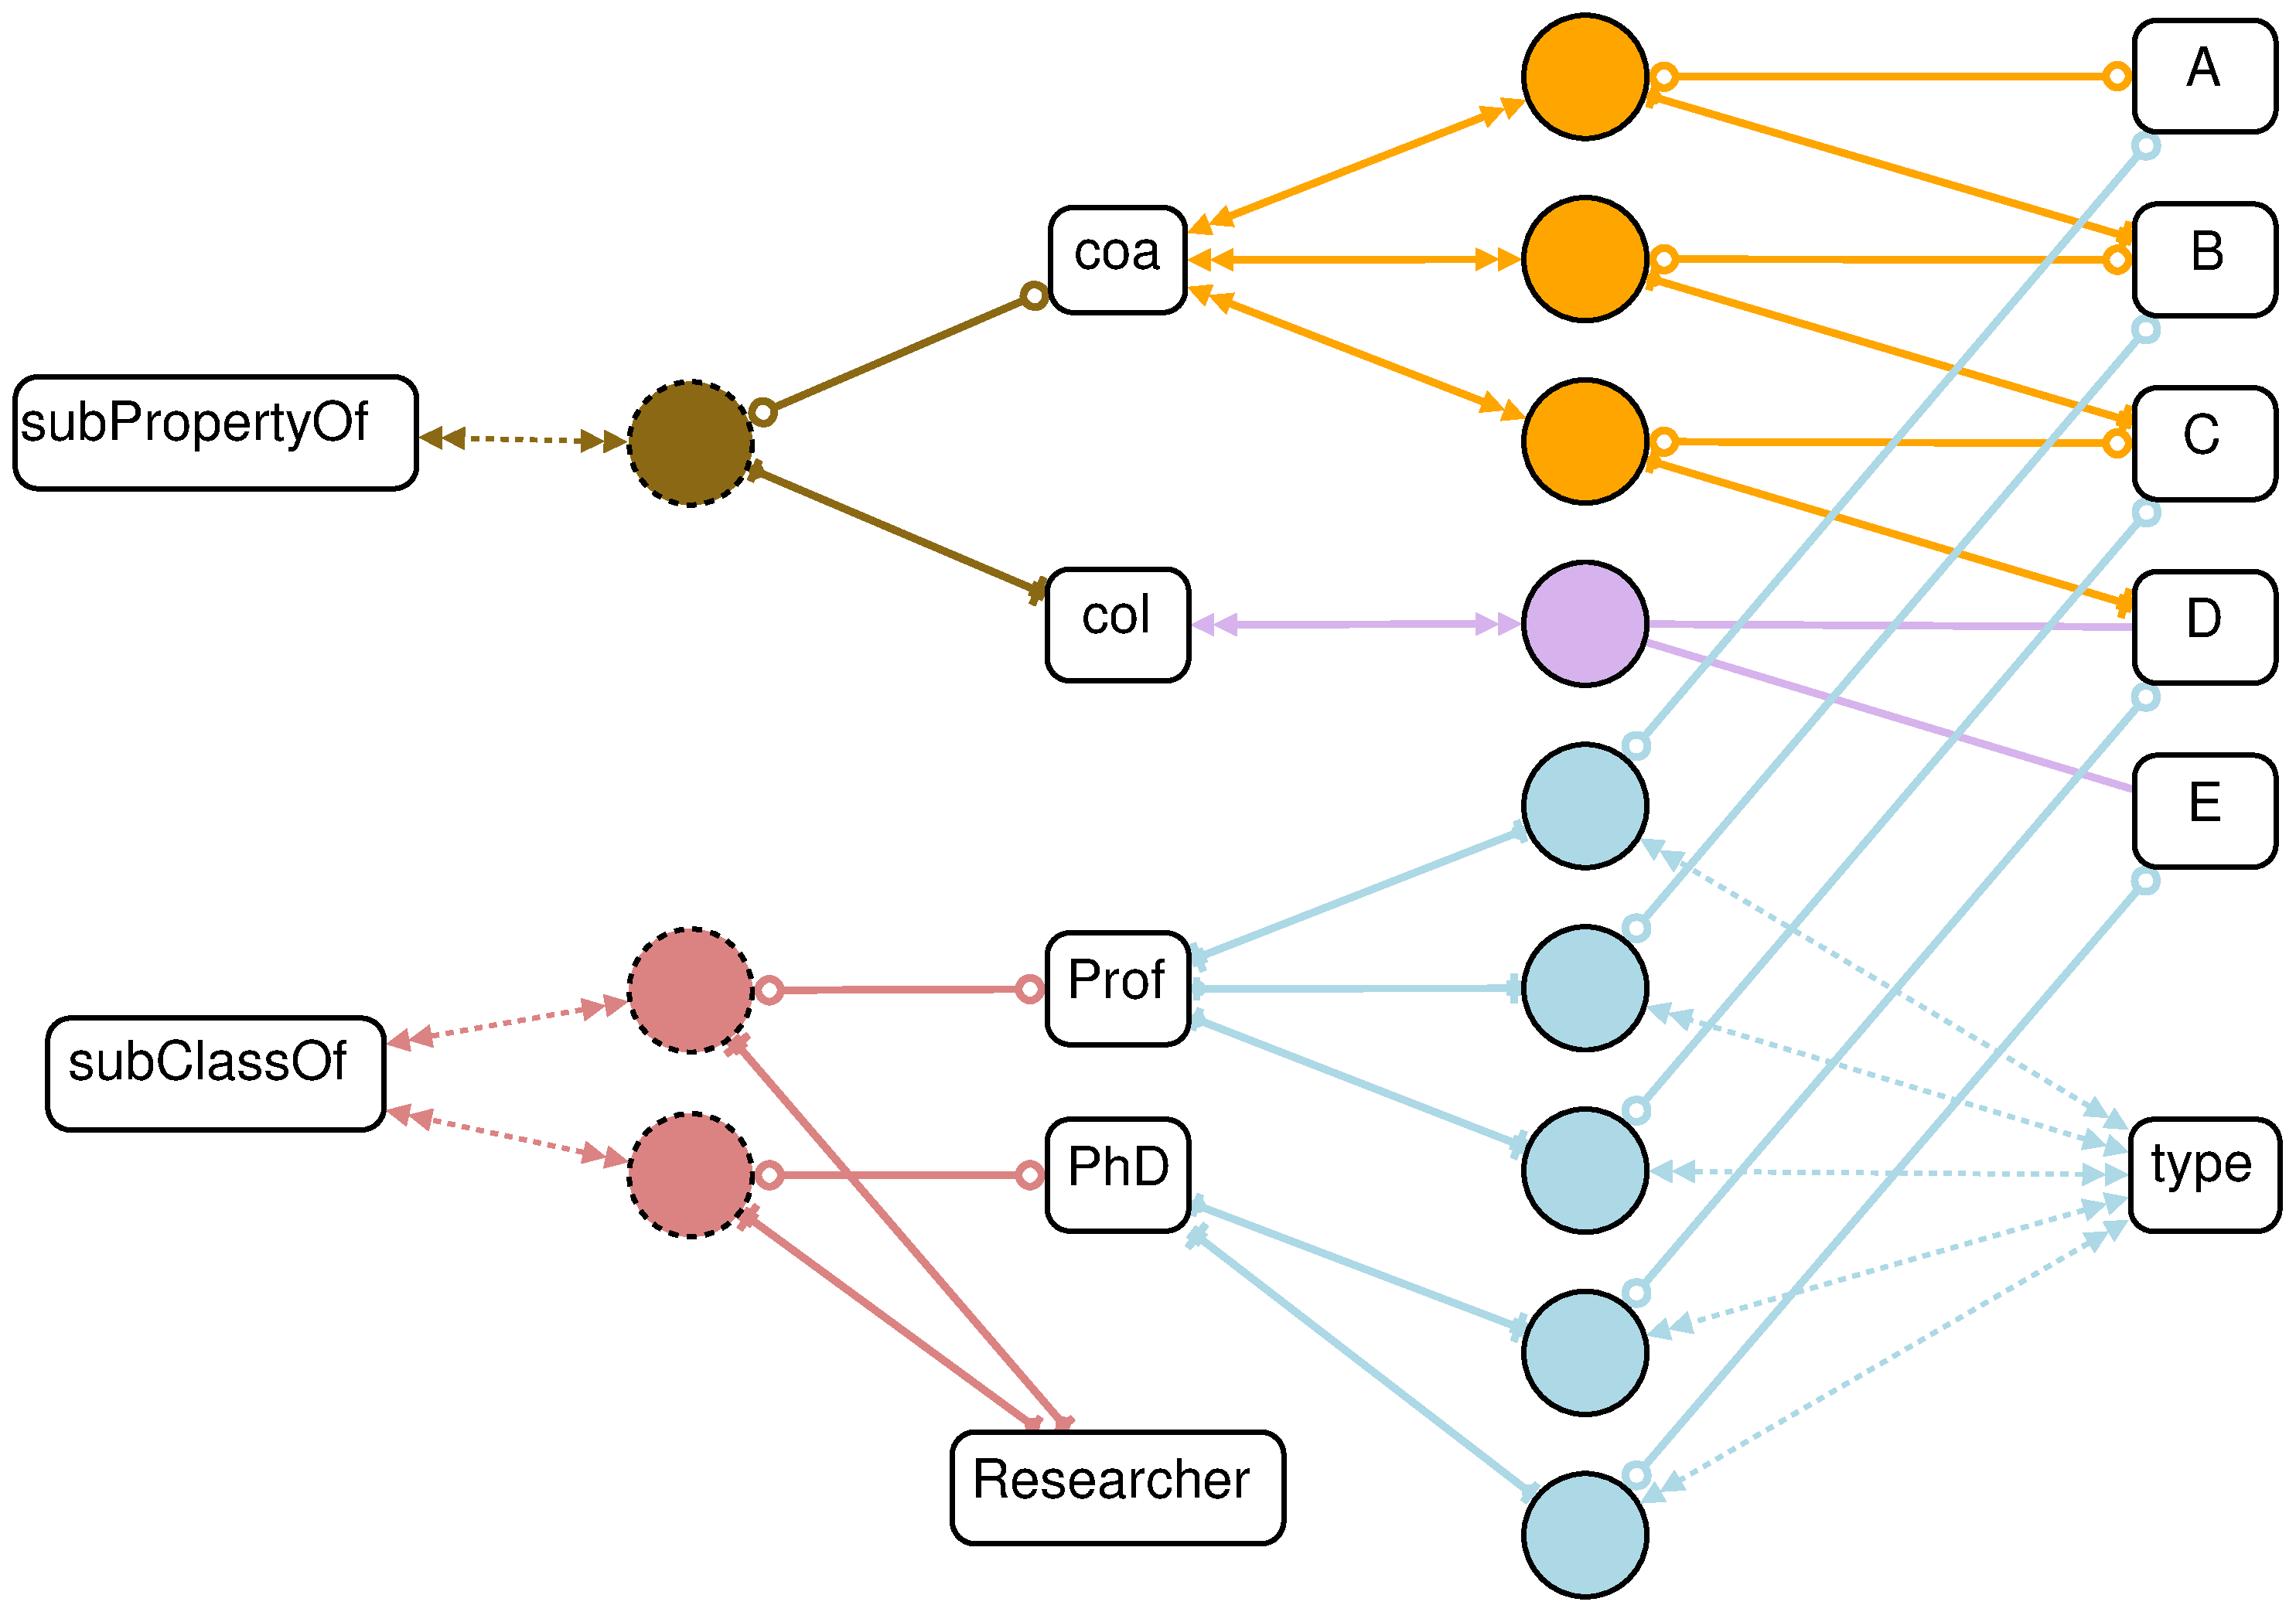
\includegraphics[width=.65\textwidth]{fig/hypergraph_mining-comp.eps}
\end{center}
\caption[An example RDF bipartite graph that represents various semantic relationships]{\label{fig:hypergraph_mining-comp} An example RDF bipartite graph that represents various semantic relationships.}
\end{figure}
